\documentclass[11pt]{article}
\usepackage{setspace}
\usepackage[a4paper,margin=1in]{geometry}
\geometry{margin=0.85in}
\setstretch{1.0}
\usepackage{graphicx}
\usepackage{array}
\usepackage{setspace}
\usepackage{parskip}
\usepackage{ragged2e}

\pagestyle{empty}
\setstretch{1.05}

\begin{document}


% Title
\begin{center}
    {\Large \textbf{Job Application}} \\[3cm]
    
    {\Huge \textbf{Zhongli Wang}} \\[0.4cm]
    
    {\huge Application for Quant Researcher}
\end{center}

\vspace{0.6cm}

% Large picture in the middle
\begin{center}
    \IfFileExists{../zhongli-wang-profile.jpg}{
        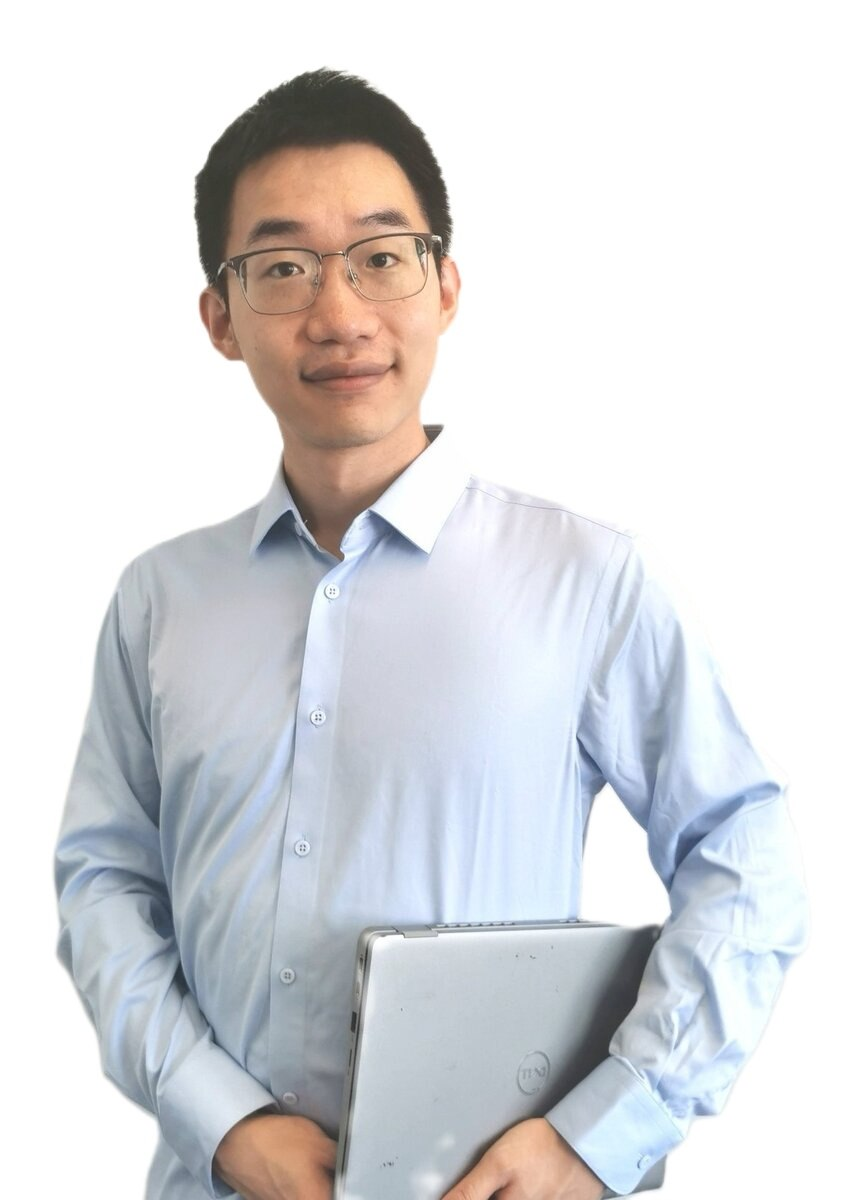
\includegraphics[
            width=0.55\textwidth,
            height=0.45\textheight,
            keepaspectratio
        ]{../zhongli-wang-profile.jpg}
    }{
        \vspace{0.45\textheight}
    }
\end{center}

\vspace{0.7cm}

% \vspace{3cm}


% Personal details
\begin{center}
\renewcommand{\arraystretch}{1.35}
\begin{tabular}{>{\bfseries}p{4.2cm} p{8.5cm}}


Address: & Astastrasse 22, 33617 Bielefeld, Germany \\

Number: & +49 160 9541 6015 \\

Email: & nkwangzhongli@gmail.com \\
\end{tabular}
\end{center}

\vfill

% \begin{center}
%     \small Last updated: \today
% \end{center}
\newpage
\enlargethispage{4\baselineskip}

\begin{flushright}
Zhongli Wang \\
+49 160 9541 6015 \\
nkwangzhongli@gmail.com \\
Bielefeld, Germany \\
\end{flushright}

\vspace{0.1cm}

\noindent
Mark Francis \\
Director \\
SilverStrand Executive Search Limited \\

\vspace{0.1cm}

\noindent
Application for Quant Researcher \\

\vspace{0.05cm}

\noindent Dear Mr. Francis,

I am writing to apply for the Quant Researcher position in Hong Kong. I am completing the final stage of my Ph.D. in Economics at Bielefeld University, with my defense scheduled for September 21, 2026, and I also hold an M.A. in Business and Economics with a Banking and Finance major and a B.Sc. in Finance. My background combines statistical modeling, Python-based computational research, financial data analysis, and clear communication across international teams.

My closest fit with this role is the discipline required to turn noisy data and model output into decisions that can be tested, monitored, and improved. In my doctoral work, I build computational models of strategic firm behavior, estimate parameters, and analyze how market structure changes outcomes under uncertainty. In a published financial-statement fraud detection project, I worked with accounting, financial, and market indicators and applied XGBoost to identify red flags in listed companies.

I would bring the following strengths to a quantitative trading research team:

\begin{itemize}
    \item \textbf{Statistical research:} Econometrics, machine learning, SMM, MCMC, and agent-based modeling for testing mechanisms in complex market environments.
    \item \textbf{Data processing:} Advanced Python skills, plus R, Julia, Mathematica, SQL basics, and experience converting financial and behavioral data into reproducible analysis.
    \item \textbf{Market-structure perspective:} Finance training and research on competition, network effects, capacity constraints, and data-driven markets.
    \item \textbf{Execution discipline:} Experience preparing models, checking assumptions, presenting results under scrutiny, and collaborating across China and Europe.
\end{itemize}

I am particularly interested in this opportunity because it combines quantitative research with implementation inside an automated trading framework. I would aim to contribute by building well-documented research pipelines, analyzing large datasets for tradable patterns, checking data and processes before market open, and monitoring strategy behavior with the caution required in live markets. I have not yet worked as a dedicated trading-desk quant, but my training is aligned with the analytical core of the role: statistical inference, programming, financial markets, and disciplined model validation.

Thank you so much for your time and consideration! I would welcome the opportunity to discuss how my research background, financial training, and coding experience can contribute to this Quant Researcher mandate.

\vspace{0.05cm}
\noindent Sincerely, \\[0.08cm]
\noindent Zhongli Wang \\[-0.2cm]

\vspace{0.1cm}
\noindent
\includegraphics[width=2.7cm,keepaspectratio]{../Wang-sig.jpg}

\end{document}
